% -*- TeX-master: "main"; fill-column: 72 -*-

\section{Proposed syntax and semantics}
\label{syntax}

In this section, we define the syntax and semantics of the Flux Balance
Constraints package for SBML Level~3 Version~1.  We expound on the various
data types and constructs defined in this package, then in \sect{examples},
we provide complete examples of using the constructs in an example SBML
model.

\subsection{Namespace URI and other declarations necessary for using this
package}
\label{xml-namespace}

Every SBML Level~3 package is identified uniquely by an XML namespace URI.
For an SBML document to be able to use a given SBML Level~3 package, it
must declare the use of that package by referencing its URI.  The following
is the namespace URI for this version of the Flux Balance Constraints
package for SBML Level~3 Version~1:
\begin{center}
\uri{http://www.sbml.org/sbml/level3/version1/fbc/version1}
\end{center}

In addition, SBML documents using a given package must indicate whether understanding the package is required for complete mathematical interpretation of a model, or whether the package is optional.  This is done using the attribute \token{required} on the \token{<sbml>} element in the SBML document.  For the \FBCPackage, the value of this attribute must be set to \val{false}.

The following fragment illustrates the beginning of a typical SBML model
using SBML Level~3 Version~1 and this version of the Flux Balance
Constraints package:

\begin{example}
<?xml version="1.0" encoding="UTF-8"?>
 <sbml xmlns="http://www.sbml.org/sbml/level3/version1/core" level="3" version="1"
   xmlns:fbc="http://www.sbml.org/sbml/level3/version1/fbc/version1" fbc:required="false">
\end{example}

\begin{figure}[h!]
  \centering
  % Requires \usepackage{graphicx}
  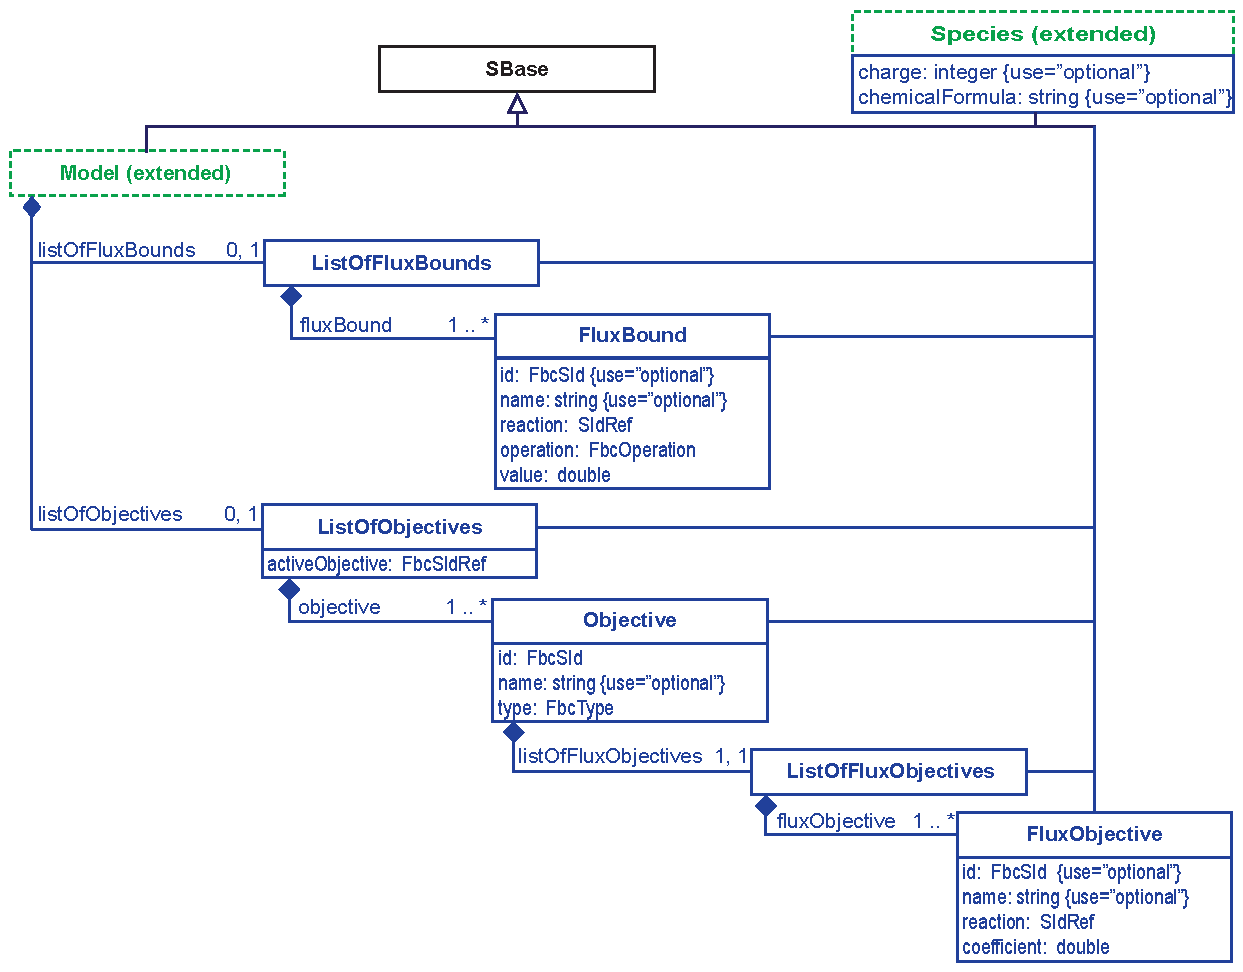
\includegraphics[width=\textwidth]{images/fbc_uml.pdf}\\
  \caption{A UML representation of the \FBCPackage. Derived from \SBase, the \FBC classes inherit support for constructs such as SBML \Notes and \Annotation's. See \ref{conventions} for conventions related to this figure. The individual classes are further discussed in the text.}
  \label{fig:fbc_uml}
\end{figure}

\subsection{Primitive data types}
\label{primtypes}

Section~3.1 of the \sbmlthreecore specification defines a number of primitive
data types and also uses a number of XML Schema 1.0 data types~\citep{biron:2000}.
More specifically we make use of \primtype{integer}, \primtype{double},
\primtype{string}, \primtype{SId} and \primtype{SIdRef}. In addition we make use of
%four new primitives \primtype{FbcSId}, \primtype{FbcSIdRef} as well as
two new primitives: the enumerations \primtype{FbcType} and \primtype{FbcOperation},
see \ref{fig:fbc_uml} for the interrelation between these entities.

The \primtype{SId} type is used as the data type for the identifiers of \FluxBound
(\ref{fluxbound-class}), \FluxObjective (\ref{fluxobjective-class}) and \Objective
(\ref{objective-class}) classes. In the FBC package the \ListOfObjectives has an
attribute of type \primtype{SIdRef} that is used to refer to an `active' \Objective.

%\subsubsection{Type \primtypeNC{FbcSId}}
%\label{primtype-fbcsid}
%
%The type \primtype{FbcSId} is derived from \primtype{SId} (\sbmlthreecore
%specification Section~3.1.7) and has identical syntax. The \primtype{FbcSId}
%type is used as the data type for the identifiers of \FluxBound
%(\ref{fluxbound-class}), \FluxObjective (\ref{fluxobjective-class}) and \Objective (\ref{objective-class}) classes. By
%using a separate identifier type we differentiate them from others defined
%in the \SBML model and thus ensuring data encapsulation.
%The equality of \primtype{FbcSId} values is determined by an exact character sequence match and therefore comparisons of these identifiers must be performed in a case-sensitive manner.

%\subsubsection{Type \primtypeNC{FbcSIdRef}}
%\label{primtype-fbcsidref}
%
%Type \primtype{FbcSIdRef} is used for all attributes that refer to identifiers of type \primtype{FbcSId}.  Derived from \primtype{FbcSId} it has the restriction that the value of an attribute having type \primtype{FbcSIdRef} must match the value of a \primtype{FbcSId} attribute in the current model. In the FBC package the \ListOfObjectives has an attribute of this type that is used to refer to an
%`active' \Objective.

\subsubsection{Type \primtypeNC{FbcType}}
\label{primtype-fbctype}

The \FBCPackage defines a new enumerated type \primtype{FbcType} which
represents the optimization sense of the objective function. It can have one
of the following two values \val{maximize} or \val{minimize}.

\subsubsection{Type \primtypeNC{FbcOperation}}
\label{primtype-fbcoperation}

The \FBCPackage defines a new enumerated type \primtype{FbcOperation} which
represents a boolean operator. It can take only one of the following values:
\val{lessEqual}, \val{greaterEqual} or \val{equal}.
%\val{less}, \val{greater}

\newpage
\subsection{The extended \class{Model} class}
\label{model-class}
\label{listoffluxbounds-class}
\label{listofobjectives-class}

The \SBML \Model class is extended with the addition of two children, i.e. a
\token{listOfFluxBounds} and a \token{listOfObjectives} and a \Model may contain at most one of these lists.

\subsubsection{The \FBC \class{listOfFluxBounds}}

As shown in \ref{fig:fbc_uml} the \ListOfFluxBounds is derived from \SBase
and inherits the attributes \token{metaid} and \token{sboTerm}, as well as
the subcomponents for \Annotation and \Notes. \ListOfFluxBounds must contain
at least one \FluxBound (defined in \ref{fluxbound-class}).

\subsubsection{The \FBC \class{listOfObjectives}}

As shown in \ref{fig:fbc_uml} the \ListOfObjectives is derived from \SBase
and inherits the attributes \token{metaid} and \token{sboTerm}, as well as
the subcomponents for \Annotation and \Notes. Unlike most other \SBML
\textsf{\textbf{ListOf\rule{0.15in}{0.5pt}}} classes, \ListOfObjectives
introduces an additional required attribute \token{activeObjective}. The
\ListOfObjectives must contain at least one \Objective (defined in
\ref{objective-class}).

\paragraph{The \token{activeObjective} attribute}
\label{activeObjective-attribute}

This attribute is of type \primtype{SIdRef} and can only refer to the
\token{id} of an existing \Objective. This required attribute exists
so that when multiple \Objective's are included in a single model, the
model will always be well described i.e. there is a single, primary
objective function which defines a single optimum and its associated
solution space.

\subsubsection{A note on units}
\label{fbcunits}
The main unit definitions that should be considered when using the \FBCPackage are the global model definitions of ``extent''  and ``time'' as all \FBC flux related classes i.e. \FluxBound and \FluxObjective implicitly attain the same unit as the \Reaction that they reference. More details on units can be found in their respective class definitions.

\subsection{The extended \class{Species} class}
\label{species-class}

The \FBCPackage extends the \sbmlthreecore \Species class with the addition
of two attributes:

\paragraph{The \token{charge} attribute}
The optional attribute \token{charge} which contains a signed
\primtype{integer} referring to the \Species object's charge and is
defined as it was in the \SBML Level 2 Version 1 specification
: \textit{``The optional field charge takes an integer indicating
the charge on the species (in terms of electrons, not the SI unit coulombs).''}

\paragraph{The \token{chemicalFormula} attribute}
\label{chemicalFormula-attribute}
The optional attribute \token{chemicalFormula} containing a
\primtype{string} that represents the \Species objects elemental
composition.
%
\exampleFile{examples/ex_spec_l3.txt}
%
While there are many ways of referring to an elemental composition the purpose of the \token{chemicalFormula} attribute is to allow reaction balancing and validation which is particularly important in constraint based models.

The format of \token{chemicalFormula} must consist only of atomic names (as in the Periodic Table) or user defined compounds either of which take the form of a single capital letter followed by zero or more lowercase letters. Where there is more than a single atom present, this is indicated with an integer. With regards to order (and enhance inter-operability) it is recommended to use the Hill system order \cite{hillsystem, hillwikipedia}.
%
\begin{table}[h!]
  %\centering
  H2O4S\qquad C2H5Br\qquad BrH\\
  C10H12N5O13P3\qquad CH3I\\
  \caption{Examples of chemical formulas written using the Hill System. As described in \ref{chemicalFormula-attribute}}\label{table:hill}
\end{table}
%
Using this notation the number of carbon atoms in a molecule is indicated first, followed by the number of hydrogen atoms and then the number of all other chemical elements in alphabetical order. When the formula contains no carbon; all elements, including hydrogen, are listed alphabetically.
%
\begin{figure}[h!]
  \centering
  % Requires \usepackage{graphicx}
  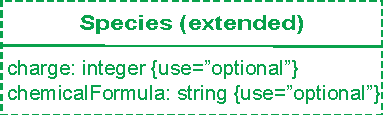
\includegraphics[width=6cm]{images/fbc_uml_species.pdf}\\
  \caption{A UML representation of the extended \SBML \Species class used in
  the \FBCPackage. See \ref{conventions} for conventions related to this
  figure.}
  \label{fig:fbc_uml_species}
\end{figure}

\newpage
\subsection{The \FBC \class{FluxBound} class}
\label{fluxbound-class}

\FluxBound is a new \FBC class derived from \SBML \SBase that inherits
\token{metaid} and \token{sboTerm}, as well as the subcomponents for
\Annotation and \Notes. The purpose of this class is to hold a single
(in)equality that provides the maximum or minimum value that a reaction flux
can obtain at steady state. It implements four attributes.

\paragraph{The \token{id} and \token{name} attributes}
A \FluxBound has two optional attributes: \token{id} an attribute of type
\primtype{SId} and \token{name} an attribute of type \primtype{string}.

\paragraph{The \token{reaction} attribute}
The required \token{reaction} attribute of type \primtype{SIdRef}. This attribute must refer to a \Reaction element defined within the enclosing model.

\paragraph{The \token{operation} attribute}
The \token{operation} attribute contains a value of type
\primtype{FbcOperation} that can take a limited set of boolean operators as
defined in \ref{primtype-fbcoperation}. The \token{operation} attribute
represents a mathematical (in)equality of the form <\token{reaction}>
<\token{operator}> <\token{value}> e.g. R$_{5}$
>= 0, R$_{5}$ <= $\infty$ and R$_{7}$ = 1.0. The mapping between traditional
mathematical symbols and \primtype{FbcOperation} values is as follows:
%
\begin{eqnarray*}
% I'm using \mapsto until I can find the proper symbol - bgoli
\label{fb-operation-enum}
 \nonumber
  <= & \mapsto & \textrm{``}\mathtt{lessEqual}\textrm{''}\\
  >= & \mapsto & \textrm{``}\mathtt{greaterEqual}\textrm{''}\\
  = & \mapsto & \textrm{``}\mathtt{equal}\textrm{''}\\
%  < & \mapsto & \val{less}\\
%  > & \mapsto & \val{greater}
\end{eqnarray*}
%
\paragraph{The \token{value} attribute}
The \token{value} attribute holds a \primtype{double} value representing the
numerical value of the flux bound. This may include an explicitly defined
$\pm\infty$ encoded as a value, e.g. \val{INF}.

\paragraph{Encoding the \FluxBound}
As described in \ref{fluxbound-class} the flux bound represents a
mathematical (in)equality of the form\\ <\token{reaction}> <\token{operator}>
<\token{value}>.\\ In SBML Level~3 Version~1 with \FBC this is encoded as:
%
\exampleFile{examples/ex_fb_fbc.txt}
%
%This example illustrates two things: the encoding of $\infty$ and that care
%should be used when selecting inequalities such as \val{less} or
%\val{greater}. While mathematically there is a difference, this difference
%is only practically relevant when working with rational arithmetic
%(solvers).
%
\begin{figure}[h!]
  \centering
  % Requires \usepackage{graphicx}
  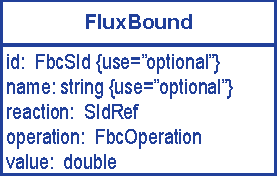
\includegraphics[width=5cm]{images/fbc_uml_fbnd.pdf}\\
  \caption{A UML representation of the \FBCPackage \FluxBound class. See
  \ref{conventions} for conventions related to this figure.}
  \label{fig:fbc_uml_fbnd}
\end{figure}
%
For an example of the how the \FluxBound relates to the description of the underlying mathematical model please see \ref{examples1:fluxbound}.

\paragraph{Units}
The \token{value} defined by the \FluxBound has the units of the \token{reaction} that it refers to i.e.~the globally defined unit of ``extent per time.''

\paragraph{Consistency of flux bounds}

It is possible, and in some cases necessary, to declare more than one
\FluxBound relating to a particular reaction. To allow as much
flexibility to the user as possible, there is no restriction on the
number of flux bounds and the operation specified by each that may be
declared for a given reaction. However, in the case where multiple
flux bounds are declared for one reaction the combined set must not
produce inconsistent values for the upper and lower bounds of the
constraint.

For example

\exampleFile{examples/ex_fb_fbc1.txt}

is obviously inconsistent since it defines \token{R >= 3} and \token{R = 2} - which
cannot be correct.

However

\exampleFile{examples/ex_fb_fbc2.txt}

would be fine since, whilst the information is essentially repeated, \token{R >= 3}
and \token{R = 3} produce the consistent result that \token{R = 3}.



\paragraph{Reactions with undefined flux bounds}
In the spirit of \sbmlthreecore the \FBCPackage does not define any default values for any element. However, in the case of a reaction with no defined flux bounds it is possible to infer this information from the reaction reversibility. In this case: irreversible reactions should be considered to be positive, $0 <= J <= \infty$ and reversible ones free/unbound, $-\infty <= J <= \infty$.

Similarly, there is also the potential for a bound to ``seemingly'' conflict with the reaction that it bounds' reversibility, e.g. a reaction is irreversible but has bounds $-\infty <= J <= \infty$. In the context of this package, flux bounds should be considered authoritative. This follows from the fact that a \FluxBound can enforce an irreversible reaction, by restricting the flux ($0 <= J <= \infty$), as well as a reversible reaction ($-\infty <= J <= \infty$). It is left to the software implementation to deal with any obvious inconsistencies.


\subsection{The \FBC \class{Objective} class}
\label{objective-class}
\label{listoffluxobjectives-class}

The \FBC \Objective class is derived from \SBML \SBase and inherits
\token{metaid} and \token{sboTerm}, as well as the subcomponents for
\Annotation and \Notes. An integral component in a complete description
of a steady-state model is the so-called `objective function' which generally
consist of a linear combination of model variables (fluxes) and a sense
(direction). In the \FBC package this concept is succinctly captured in the
\Objective class.

\paragraph{The \token{id} and \token{name} attributes}
An \Objective has a required attribute \token{id} of type
\primtype{SId} and an optional attribute \token{name} of type \primtype{string}.

\paragraph{The \token{type} attribute}
The required \token{type} attribute contains an \primtype{FbcType} type
which represents the sense of the optimality constraint and can take one of
two values:
\begin{eqnarray*}
% I'm using \mapsto until I can find the proper symbol - bgoli
\label{obj-type-enum}
 \nonumber
  maximize & \mapsto & \textrm{``}\mathtt{maximize}\textrm{''}\\
  minimize & \mapsto & \textrm{``}\mathtt{minimize}\textrm{''}
\end{eqnarray*}

\paragraph{The \token{listOfFluxObjectives} element}
The element \token{listOfFluxObjectives} which contains a
\ListOfFluxObjectives is derived from and functions like a typical \SBML
\textsf{\textbf{ListOf\rule{0.15in}{0.5pt}}} class with the restriction that it
must contain one or more elements of type \FluxObjective (see \ref{fluxobjective-class}).
This implies that if an \Objective is defined there should be at least
one \FluxObjective contained in a \ListOfFluxObjectives.
% bgoli: to me this makes sense but are there other examples of this in SBML or is everything always optional

\begin{figure}[h]
  \centering
  % Requires \usepackage{graphicx}
  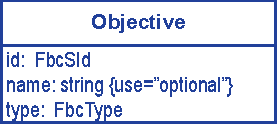
\includegraphics[width=5cm]{images/fbc_uml_obj.pdf}\\
  \caption{A UML representation of the \FBCPackage \Objective class. See
  \ref{conventions} for conventions related to this figure.}
  \label{fig:fbc_uml_obj}
\end{figure}

\paragraph{Encoding the \Objective}
The \FBCPackage allows for the definition of multiple model objectives with
one being designated as active (see \ref{objective-class}) as illustrated in
this example:
%
\exampleFile{examples/ex_objf_fbc.txt}
%
Note how both \Objective instances differ in \token{type} and each contains
different set of \class{FluxObjectives} (see \ref{fluxobjective-class}).
For an example of the how the \Objective relates to the description of the underlying mathematical model please see \ref{examples1:objfunc}.

\subsection{The \FBC \class{FluxObjective} class}
\label{fluxobjective-class}

The \FBC \FluxObjective class is derived from \SBML \SBase and inherits
\token{metaid} and \token{sboTerm}, as well as the subcomponents for
\Annotation and \Notes.

The \FluxObjective class is a relatively simple container for a model
variable weighted by a signed linear coefficient.

\paragraph{The \token{id} and \token{name} attributes}
A \FluxObjective has two optional attributes: \token{id} an attribute of type \primtype{SId} and \token{name} an attribute of type \primtype{string}.

\paragraph{The \token{reaction} and \token{coefficient} attributes}
The required \token{reaction} is of type \primtype{SIdRef} and is restricted to refer only to a \Reaction while the \token{coefficient} attribute holds a \primtype{double} referring to the coefficient that this \FluxObjective takes in the enclosing \Objective. For example the objective \texttt{ Maximize: 1 R1 + 2 R2} would be encoded as
%
\exampleFile{examples/ex_fluxobj_fbc.txt}
%
\begin{figure}[h]
  \centering
  % Requires \usepackage{graphicx}
  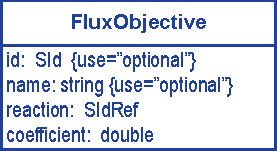
\includegraphics[width=5cm]{images/fbc_uml_fobj.pdf}\\
  \caption{A UML representation of the \FBCPackage \FluxObjective class. See
  \ref{conventions} for conventions related to this figure.}
  \label{fig:fbc_uml_fobj}
\end{figure}

\paragraph{Units}
As described above the \FluxObjective defined here as $n\cdot J$ where the \token{coefficient} ($n$) is dimensionless and the \token{value} ($J$) takes the units of the \token{reaction} flux i.e.~``extent per time''. Therefore, the \FluxObjective ($n\cdot J$)  has the unit ``extent per time'' where the units of reaction ``extent'' and ``time'' are defined globally.


